%!TEX root = ../template.tex
\chapter{State of the art and related work}
\label{cha:state_art}
This chapter will start by covering the different approaches available commercially to track players in different sports, like basketball, football, baseball, tennis and american football. Then the sensors used to measure this movements and the communication technologies used to transmit that data are described, and finally the scientific related work in the same area is presented.

\section{Different Approaches} % (fold)
\label{sec:approaches}
In this subchapter, I will describe the most common approaches used nowadays to track players in team sports (video tracking versus sensor tracking) and also the commercial applications that are available in the market.

There are two main approaches when tackling the problem of tracking players and the ball during a sports game. The first one I’ll address is a system that uses video tracking. The second is using sensors attached to the players body. 


\subsection{Video Tracking System Approach}
\label{subsec:video_approach}
\subsubsection{Cameras}
\label{subsubsec:cameras}
Camera systems are widely used in sports and can accurately track the players of both teams and the ball. One example of this system is Stats SportVU, which is used in various sports, like soccer~\cite{stats_football} and basketball~\cite{stats_basketball}, and by analyzing the video using machine learning techniques can provide statistics like distance traveled, average and maximum speeds, number of speeds, field coverage, team formation and many others. A representation of this system is shown in Figure~\ref{fig:cameras}

\begin{figure}[htbp]
  \centering
  \includegraphics[width=0.5\linewidth]{cameras}
  \caption{SportVU cameras in a basketball court~\cite{stats_basketball}}
  \label{fig:cameras}
\end{figure}

Second Spectrum, the official optical tracking provider for NBA~\cite{secondspectrum}), uses cameras located around the court to collect 3D spatial data of players and the ball like position and movements, and to gather data like speed, distance, shoots, passes, drives and many more ~\cite{secondspectrumaws}. Then, using machine learning algorithms, players and coaches can get detailed reports and insights about player performance. This approach can also be profitable for leagues and media, providing data to interactive applications or using augmented reality video to improve the fan experience.

In Football, video tracking systems are used in the VAR (Video Assistant Referees) system used by FIFA~\cite{fifavar}, which reviews the decisions made by the referee using video footage of the game. A video system is also used for the Goal-line Technology, to detect if the whole of the ball has crossed the goal line~\cite{fifagoalline}.

Baseball uses a system called Hawk-eye, that enables teams to make in-game decisions, like deciding when to challenge a call. This system uses 15 cameras, giving the team various angles to take an informed decision~\cite{hawkeyebaseball}.

Hawk-eye technologies are used in over 80 Tennis Tournaments to track close line calls, like foot faults or to accurately identify if a ball bounced in or out of the field~\cite{hawkeyetennis}.

Videobserver is a match analysis service that joins the performance data inserted by the coach with recorded video, in order to provide a deferred statistical report of the matches. It is used mainly by football teams, but can be applied to handball, basket or hockey~\cite{videobserver}.

Video tracking systems can give very accurate measurements about the players location and team tactics, and even track small movements like shoots and passes in Basketball. However, these systems require high processing power, and are very expensive, being out of reach for minor and amateur teams. Video systems are also attached to the field, and in order to track a team in a different location, the system needs to be installed there. Another drawback is that some video systems don’t work in real-time. They need an operator to tag events, and the processed data is deferred.

\subsection{Sensor Based Tracking Systems}
\label{subsec:sensor_approach}
The sensor approaches usually combine the use of a positioning system like a GNSS (Global Navigation Satellite System) or a Radio Frequency positioning system like Ultra-Wide Band or RFID (Radio Frequency Identification and IMU (Inertial Measuring Unit) sensors. An IMU is a device that measures orientation, velocity and forces using accelerometers, gyroscopes and magnetometers.

For tracking soccer players, a high number of teams use STATSports Apex, a tracking device that includes GPS, accelerometer, gyroscope and magnetometer, and communicates using Bluetooth Low Energy. It is used by over 280 teams in Europe, 60 in the North America and 70 in the rest of the world~\cite{statsports_clients}. 

By using Bluetooth LE, this device can connect simultaneously to hearth rate sensor, smart watches and mobile devices, gathering all the data and becoming the center of a body network, and this data can be transferred, stored and accessed online, providing over 25 insightful metrics, like total speed or number of accelerations~\cite{statsports_apex}. 

For positioning, this system uses GPS combined with Ultra-Wide Band (UWB) positional beacons. For outdoor or stadium environments, GPS is used, combined with 2 positional beacons to enhance the GPS position. For indoor environments, at least 4 UWB beacons are used for providing accurate positioning~\cite{statsports_mapps}.

In NBA, wearable devices aren’t allowed in game nights. However, these sensors are used in training situations. Kinexon~\cite{kinexon} is a widely used system in basketball teams. Kinexon uses an Ultra-Wide Band Radio system to accurately measure the location of the players, based on the time-of-arrival of the signal sent by a beacon used by the players~\cite{ghentuwb}. 

In the National Football League (NFL), Zebra~\cite{zebranfl} uses RFID tags on the players shoulder pads to track and to provide analytics to coaches, players and fans.

Sensor based tracking systems are more portable and provide teams and players more freedom in changing the playing court. They are typically cheaper, making it accessible to amateur teams. These systems track load and motion metrics like the covered distance, but lack basketball specific metrics like shoots and passes. These systems also need an outside infrastructure to be able to position the players, either by \gls{GPS} or Ultra-Wide Band antennas around the court. 

Our solution fits the sensor-based tracking system category, but we aim to track the position player and gather basketball game metrics only using inertial sensors.

\section{Sensors} % (fold)
\label{sec:sensors}
A sensor is a device that detects or measures a physical property, and converts that value to an electric signal, which is usually transmitted to a processing unit. The input can be something like light, heat, motion, pressure, moisture, and many other physical or chemical phenomenon. %%sustentar esta definição

A wide variety of different sensors are used in sport applications, to track the players. We are going to divide this in two main classes: a general overview of data acquisition sensors used in sports and focus on the sensors used to track position and motion~\cite{ubiquitoussports}. 


\subsection{Data Acquisition Sensors in Sports}
\label{subsec:data_sensors}
%%o que é interessante medir em desportos de equipa
\subsubsection{Body Temperature}
\label{subsubsec:body_temp}
In order to prevent body injuries (or in extreme cases, death), the body core temperature should be around 37 °C. The most accurate widely used techniques for measuring athletes core temperature are highly-invasive, like rectal probing or ingesting pills. The most adopted way to unobtrusively measure the core temperature of athletes is using the tympanic temperature inside the ear~\cite{tympanic}. An example of a tympanic measuring device developeb by Cosinuss~\cite{cosinuss} is shown in Figure~\ref{fig:ear}.

\begin{figure}[htbp]
  \centering
  \includegraphics[width=0.5\linewidth]{cosinuss}
  \caption{Cosinuss tympanic measuring device~\cite{cosinuss}}
  \label{fig:ear}
\end{figure}

\subsubsection{Hearth Rate}
\label{subsubsec:hearth_rate}
There are two main methods to measure the hearth rate: Electrocardiography (ECG) and Photoplethysmography (PPG)~\cite{ppgreview}.

The first one uses electrodes placed on the skin (preferentially on the chest) to measure the electrical activity of the hearth. Hexoskin~\cite{hexoskin} uses this method, as shown in Figure~\ref{fig:ecg_round}. The second one uses light to detect the change in blood vessels sensing the pulse, as shown in Figure~\ref{fig:ppg}. The latter is commonly used in smartwatches, placed on the wrist~\cite{ppgsmartwatch}. 

\begin{figure}[htbp]
  \centering
  \subcaptionbox{ECG device~\cite{hexoskin} \label{fig:ecg_round}}%
    {\includegraphics[width=0.5\linewidth]{ecg}}%
  \subcaptionbox{PPG device~\cite{apple_watch} \label{fig:ppg}}%
    {\includegraphics[width=0.5\linewidth]{ppg}}%
  \caption{Hearth Rate measuring devices}
  \label{fig:hearthrate}
\end{figure}

\subsubsection{Insole Pressure Sensors}
\label{subsubsec:pressure}
Pressure sensors incorporated in the insole can provide critical information in medical diagnostics, rehabilitation and sports performance analysis~\cite{insole}.

Companies like Moticon~\cite{moticon} or FeetMe~\cite{feetme} provide insoles equipped with wireless sensors that can provide in real-time metrics as gait timing, balance, pressure points, applied force and motion for both feet.
Figure~\ref{fig:pressure} shows the product commerciallized by Moticon.

\begin{figure}[htbp]
  \centering
  \includegraphics[width=0.5\linewidth]{moticon}
  \caption{Moticon insole pressure sensors~\cite{moticon}}
  \label{fig:pressure}
\end{figure}


\subsubsection{Perspiration}
\label{subsubsec:perspiration}
UC Berkley is developing a sweat wearable sensor, that can measure metabolites and electrolytes in sweat, calibrate this data based on skin temperature (because temperature can alter the response of some sensors) and send this data wirelessly to a smartphone. This data can analyze continuous and non-invasively the user’s fatigue, hydration and body temperature~\cite{berkleysweat}.

\subsubsection{Respiration}
\label{subsubsec:respiration}
Respiration rate is often obtained by measuring the change in thoracic volume using a chest mounted strap, shown in Figure~\ref{fig:resp}, equipped with a stretch sensor that measure the expansion or contraction of the rib cage~\cite{respiration1} or a piezoelectric sensor to measure the displacement variations provoked by inhalation or exhalation~\cite{respiration2}.

\begin{figure}[htbp]
  \centering
  \includegraphics[width=0.5\linewidth]{respiration}
  \caption{Respiration measuring strap~\cite{respiration1}}
  \label{fig:resp}
\end{figure}

\subsubsection{VO2 Max}
\label{subsubsec:vo2}

VO2 max stands for maximum volume of O2 consumed (i.e. the body’s ability to supply the muscles oxygen through the blood), often measured in laboratories from peak work rate achieved on a treadmill, using masks to capture every molecule of oxygen inhaled and exhaled~\cite{vo2lab}.

To estimate VO2 max, wearing a face mask isn’t within the capability of a smartwatch or smart band. Most consumer wearables use an estimation provided by a company called Firstbeat~\cite{firstbeat}, which claims to be 95\% accurate when compared to laboratory measurements, according to the company’s white paper~\cite{firstbeatwhite}.

This estimation considers the weight, sex and age of the user, and using fixed tests like the Cooper test or the Rockport walk test collects hearth rate and speed. The collected data is segmented, and its reliability is calculated. Then, the most reliable data segments are used to estimate the users VO2 max.


%%%%%%%%%%%%%%%%%%%%%%%%%%%%%%%%%%%%%%%%%%%%%%%%%
\subsection{Motion Sensors}
\label{subsec:motion_sensors}

\subsubsection{Accelerometer}
\label{subsubsec:accelerometer}
Accelerometers measure acceleration forces, which is the rate of change of the velocity of an object, with respect to time. The unit used to acceleration is meter per second squared (m/s2), or G-forces (g). On planet Earth, at sea level, 1 g is equivalent to 9,8 m/s2. This value changes slightly with altitude, and will be different on different planets, because of different planet masses.

Accelerometers are useful to measure vibrations, movements and orientation, and can measure static forces, like gravity, or dynamic forces, like moving the sensor.

There are two main ways to measure these forces. Usually accelerometers use capacitive plates, either fixed or attached to springs, and the change of position between these plates changes de capacitance between them. This change is measured and converted into acceleration, as shown in Figure~\ref{fig:acc_cap}. Other way is to use the piezo-electric effect. These accelerometers have microscopic crystal structures can output electrical charge when put under stress, like an acceleration force, as shown in Figure~\ref{fig:acc_piezo}~\cite{accelerometerspark}~\cite{accelerometerde}~\cite{accelerometerglobal}.

\begin{figure}[htbp]
  \centering
  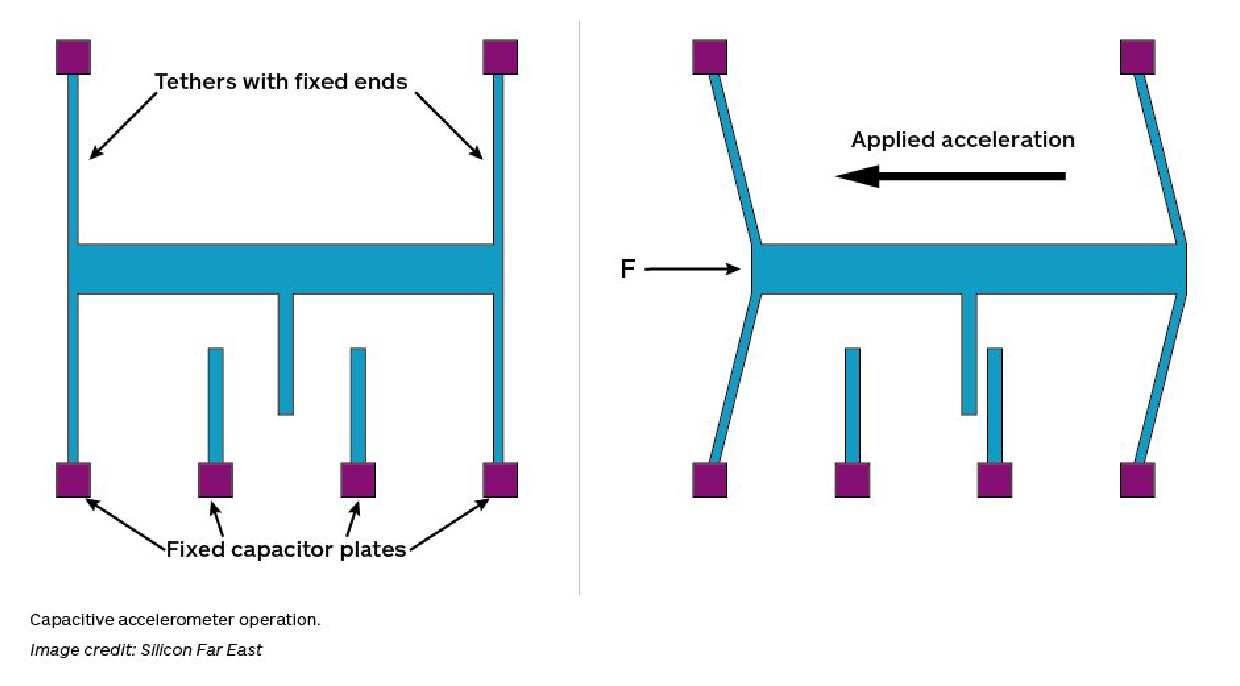
\includegraphics[width=1\linewidth]{accelerometer_cap}
  \caption{Capacitative accelerometer sensor~\cite{accelerometerglobal}}
  \label{fig:acc_cap}
\end{figure}

\begin{figure}[htbp]
  \centering
  \subcaptionbox{Withouth applied force\label{fig:acc_piezo1}}%
    {\includegraphics[width=0.5\linewidth]{accelerometer_piezo_1}}%
  \subcaptionbox{With applied force\label{fig:acc_piezzo2}}%
    {\includegraphics[width=0.5\linewidth]{accelerometer_piezo_2}}%
  \caption{Piezo accelerometer sensor~\cite{accelerometerspark}}
  \label{fig:acc_piezo}
\end{figure}


\subsubsection{Gyroscope}
\label{subsubsec:gyroscope}
Gyroscopes are devices used to measure and maintain orientation and angular velocity.
%[https://www.lexico.com/en/definition/gyroscope]
There are various classes of gyroscopes, used for different needs of performance, cost and volume: mechanical gyroscopes, optical gyroscopes and Micro-electromechanical system (MEMS) gyroscopes~\cite{gyro1}.

The most adopted class of gyroscopes for consumer use is the MEMS gyroscopes, due to their low cost and low performance. The unit used to measure angular velocity is degrees per second (º/s). MEMS gyroscopes usually use a vibrating mechanical element to determine the rate of rotation, in 1, 2 or 3 axes~\cite{gyrospark}.


Most MEMS gyroscope take advantage from the Coriolis effect to measure angular velocity. Using a tuning fork configuration, where two masses vibrate constantly in opposite directions, when these masses experience an angular velocity (rotation), the Coriolis force acts on each mass in opposite directions, resulting on a change of capacitance, which is measured to calculate the rate of rotation~\cite{gyromems}. This effect is shown in Figure~\ref{fig:gyro}.

\begin{figure}[htbp]
  \centering
  \includegraphics[width=0.5\linewidth]{gyroscope}
  \caption{Gyroscope sensor~\cite{gyromems}}
  \label{fig:gyro}
\end{figure}

\subsubsection{Magnetometer}
\label{subsubsec:magnetometer}
A magnetometer is a device used to measure the strength and the direction of magnetic fields. The most common method for measuring magnetic fields is using the Hall Effect.  If we have a conductive plate, the electrons would flow from one end to the other. Bringing this plate near to a magnetic field, the electrons would deflect to one side or the other of the plate. Putting a meter between the two sides, the voltage would change accordingly to the direction and strength of the magnetic field, as shown in Figure~\ref{fig:magnetometer}.

This effect can be used to measure the Magnetic North of the Earth, providing handheld devices a sense of orientation in relation to Earth. However, these small magnetometer measurements are easily disturbed by nearby objects, like a computer or a Wi-Fi router, which makes this device unreliable~\cite{magnetometer1}~\cite{magnetometer2}.

\begin{figure}[htbp]
  \centering
  \includegraphics[width=0.5\linewidth]{magnetometer}
  \caption{Magnetometer sensor~\cite{magnetometer1}}
  \label{fig:magnetometer}
\end{figure}

\subsubsection{GNSS}
\label{subsubsec:gnss}
GNSS stands for Global Navigation Satellite System, which is a system that provides autonomous geo-spatial, and allows small electronic devices to determine their location precisely. This location is expressed in longitude, latitude and altitude.

There are three GNSS systems available for civilian use: Galileo, developed by the Europe Union, GLONASS, developed by Russia and GPS, developed by the United States of America~\cite{gnss1}. The latter is the most widely used. It was developed to accurately determine the absolute position on Earth, initially for military purposes, but soon was publicly released.

This system is divided into three segments:
\begin{itemize}
  \item Space Segment – 24 satellites orbiting the earth
  \item Control Segment – 5 ground stations positioned on the earth’s equator to control the Space Segment
  \item User Segment – any user that receives the GPS signal
\end{itemize}

Triangulation is used to accurately position the user, using at least 4 satellites to obtain position and time correctly, as shown in Figure~\ref{fig:gnss}~\cite{gnss2}.

\begin{figure}[htbp]
  \centering
  \includegraphics[width=0.5\linewidth]{gps}
  \caption{GNSS System~\cite{gnssimg}}
  \label{fig:gnss}
\end{figure}



%%%%%%%%%%%%%%%%%%%%%%%%%%%%%%%%%%%%%
\section{Communication Protocols}
\label{sec:communication_protocols}
In order to communicate with the sensors, and to collect the data, a communication layer is needed. In this chapter the main communication protocols are presented and compared, in order to find the protocol that best suits the system requirements.

\subsection{Protocols}
\label{subsec:protocols}

\subsubsection{Cellular}
\label{subsubsec:cellular}
Cellular technology is meant to use cases where the need of data throughput is high, there is a big distance to cover and there are low restraints on power consumption.
Using GSM/3G/4G (and soon 5G), peak data rates can reach up to 20Gbps \cite{5g}. Cellular communication protocol is meant to applications in mobile devices. 

\subsubsection{SigFox}
\label{subsubsec:sigfox}
SigFox builds wireless networks to connect low power objects and devices, which are continuously turned on and send small amounts of data.
SigFox uses Ultra Narrow Band modulation and communicates at 100 or 600 bits per second \cite{sigfox}. 
SigFox is complementary with other technologies, like Bluetooth, GPS, Cellular and Wi-Fi, unleashing the applications of this technology.

\subsubsection{6LoWPAN}
\label{subsubsec:6lowpan}
6LoWPAN comes from the combination of IPv6 and Low Power Wireless Personal Area Network and aims to define the IPv6 to low data rates, low power and small footprint applications, providing an adaptation layer between the MAC and the network layer (IPv6)~\cite{6lowpan2}. 
It supports different types of topologies, like star and mesh~\cite{6lowpan}. An example of an application using 6LoWPAN is shown in Figure~\ref{fig:6lowpan}.

\begin{figure}[htbp]
  \centering
  \includegraphics[width=0.5\linewidth]{6lowpan}
  \caption{6LoWPAN Topology Example~\cite{6lowpan2}}
  \label{fig:6lowpan}
\end{figure}


\subsubsection{NFC}
\label{subsubsec:nfc}
Near Field Communication is a very short-range (0-10cm) wireless protocol, establishing wireless connections between network appliances and consumer electronic, carrying very low amounts of data (424 Kbits/second).
Some examples are touching the pay terminal with the NFC-enabled phone to authorize the payment, as shown in Figure~\ref{fig:nfc}, or connecting electronic devices, like a smartphone and a headset. \cite{nfc}

\begin{figure}[htbp]
  \centering
  \includegraphics[width=0.4\linewidth]{nfc}
  \caption{NFC Payment~\cite{nfcimg}}
  \label{fig:nfc}
\end{figure}

\subsubsection{ZigBee}
\label{subsubsec:zigbee}

ZigBee is a widely used IoT protocol with different applications in the areas of home automation, offices and healthcare systems.
The networks can be configured in multiple topologies, like star, mesh and cluster tree, and consists in three types of devices: end device, router and coordinator~\cite{zigbee}~\cite{protocols}.

\begin{itemize}
  \item The coordinator is the most capable device, responsible for starting and maintaining the network, store security keys and connect with other networks. 
  \item Router devices can run applications just like de end devices, but additionally can pass information from other devices and extend the network.   
  \item End devices are the simplest and less expensive devices, can only talk to another device, but are able to sleep and to save more power than router or coordinator devices.
\end{itemize}

These topologies are illustrated in Figure~\ref{fig:zigbee}.

\begin{figure}[htbp]
  \centering
  \includegraphics[width=0.6\linewidth]{ZigBee_Topologies}
  \caption{ZigBee topologies~\cite{zigbee}}
  \label{fig:zigbee}
\end{figure}


\subsubsection{Z-Wave}
\label{subsubsec:zwave}
Z-Wave is a protocol designed for reliable wireless communication in a low power system. Developed mainly for home automation uses, connects 30-50 nodes and has a point-to-point range of 30 meters.  Its data throughput is low (100 Kbps) but is suitable for small messages like light and energy control in household environments, as shown in Figure~\ref{fig:zwave}~\cite{protocols}~\cite{zwave}.

\begin{figure}[htbp]
  \centering
  \includegraphics[width=0.5\linewidth]{zwave}
  \caption{ZWave home application~\cite{zwave}}
  \label{fig:zwave}
\end{figure}

\subsubsection{Wi-Fi}
\label{subsubsec:wifi}
Wi-Fi is a wireless technology that takes advantage of electromagnetic radiation (radio waves), operating in the 2.4GHz and 5 GHz frequencies, to connect mobile computers and network enabled devices like smartphones and IoT devices to local networks and the Internet. The name Wi-Fi is the brand name adopted by the Wi-Fi Alliance~\cite{wifi1}, which holds the Wi-Fi trademark, and certifies products to use this technology. 

Wi-Fi technology is based on the Institute of Electrical and Electronics Engineers (IEEE) wireless communication standard 802.11, which has been around for over 20 years, with various different versions of the protocol. 
The currently used version is IEEE 802.11ac (Wi-Fi 5), presenting faster and more scalable capabilities than the previous version (802.11n), allowing more bandwidth, faster speeds and lower power usage for each user~\cite{wifi2}. 

Regarding IoT, IEEE 802.11 Working Group defined the 802.11ah specification that operates in the sub-1-GHz frequency and supports a greater number of devices per access point, longer transmission range and lower data rate, and is targeted to sensors and IoT applications, competing with Bluetooth technology~\cite{wifi3}~\cite{wifi4}.

\subsubsection{Bluetooth}
\label{subsubsec:bluetooth}
Bluetooth is a low power wireless technology for exchanging data between mobile devices over short distances.

Bluetooth is managed by Bluetooth Special Interest Group (SIG), which develops, licenses and holds the trademark. To be able to use Bluetooth, a device manufacturer must meet the Bluetooth SIG standards~\cite{blesig}.

There are two types of Bluetooth technologies: 
\begin{itemize}
  \item Basic Rate/Enhanced Data Rate (BR/EDR) 
  \item Low Energy (BLE).  
\end{itemize}
While BR/EDR data rates and bandwidth are bigger and support higher data streams like audio streaming, BLE has a lower latency and lower power consumption, which is ideal for small IoT devices that only transfer small data packages at a time, as shown in Table~\ref{tab:hla:bluetooth_comparison}~\cite{ble1}.


\begin{table}[ht]
  \caption{Bluetooth Comparison}
  \label{tab:hla:bluetooth_comparison}
  \centering
  \begin{tabular}{lcc}
    \toprule
    \multicolumn{1}{c}{\textbf{Technology}} & \textbf{BR/EDR} & \textbf{BLE} \\
    \midrule
    Setup Time & 100 ms & < 6 ms \\
    Data Rate & 125 Kb/s to 2 Mb/s & 1 Mb/s to 3 Mb/s \\
    Power Consumption & 1 (Reference value) & 0.1 to 0.5 \\
    \bottomrule
  \end{tabular}
  \end{table}

Bluetooth network topologies can be of different types:
\begin{itemize}
\item \textbf{Point-to-point (1:1) -} Point-to-point network topology is used for connecting devices one-to-one. In BR/EDR this type of communication is optimized for audio streaming, like headsets, speakers or free-hands systems. In BLE, this topology is optimized for data transfer with devices like fitness trackers and PC peripherals.
\item \textbf{Broadcast (1:m) -} Broadcast establishes one-to-many connections and is only available in BLE. This topology is optimized for local information sharing, like point-of-interest information, indoor navigation and asset tracking.
\item \textbf{Mesh (m:n) -} Mesh establishes many-to-many device connections and is only available in BLE. This type of topology is useful when a large number of devices are present and need a trustworthy and safe connection network, like a building with automatic lighting functions or a sensor network. Mesh networks can span a very large physical area. This is particularly useful when a device relies on data from another device that is not in his direct range.
\end{itemize}

These topologies are illustrated in Figure~\ref{fig:bletopologies}.

\begin{figure}[htbp]
    \centering
    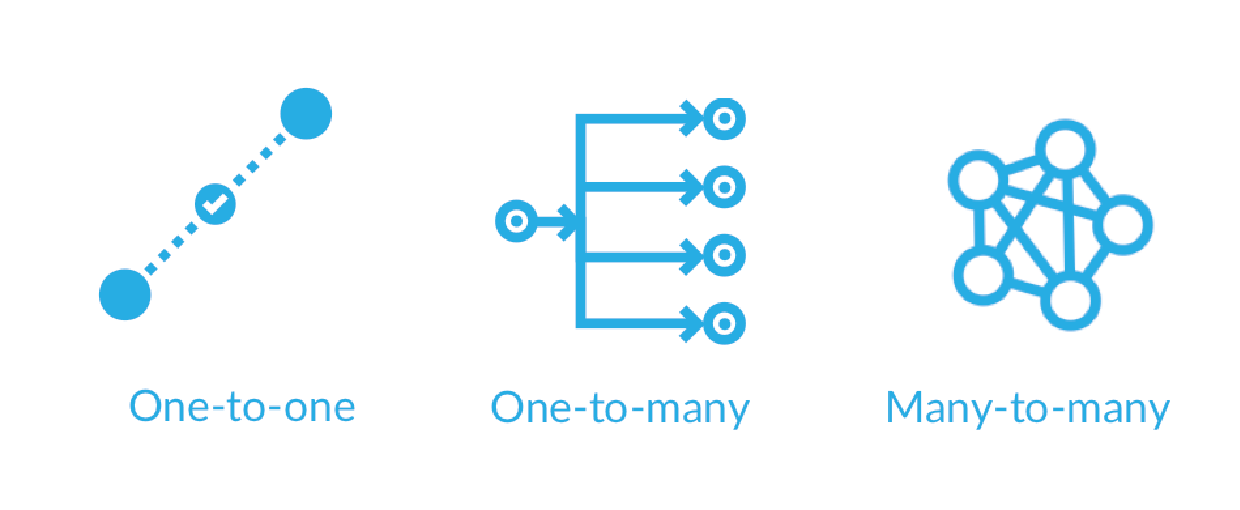
\includegraphics[width=0.8\linewidth]{ble_topologies}
    \caption{BLE Topologies~\cite{ble_mesh_topologies}}
    \label{fig:bletopologies}
\end{figure}


\subsection{Communication Protocols Comparison}
\label{subsec:comparison}

Table~\ref{tab:hla:communication_comparison} shows a comparison of the communication protocols mentioned above, regarding the frequency used, the maximum data rate, the range, the power usage and the cost of the technologies~\cite{comparison}.

In order to meet the requirements, a low power and low-cost device is needed, with a medium range (enough to cover a basketball court), and a data throughput capable of handling rates of 20-50 Hz. 

BLE is the technology that meets most of these requirements and is the technology that will be used in the following phases of this work. Besides meeting the requirements, this choice has in consideration other factors: Bluetooth is a technology that I had worked before and the sensors available in the beginning of this work were equipped with BLE technology. 

\begin{table}


\caption{Communication Protocol comparison}
\label{tab:hla:communication_comparison}
\centering
\resizebox{\textwidth}{!}{%
\begin{tabular}{lccccc}
  \toprule
  \multicolumn{1}{c}{\textbf{Technology}} & \textbf{Frequency} & \textbf{Max Data Rate} & \textbf{Range} & \textbf{Power Usage} & \textbf{Cost} \\
  \midrule
  Cellular (4G)                           & Cellular Bands     & 100 Mbps               & Several Km     & High                 & High          \\
  SigFox                                  & < 1 GHz            & < 1 kbps               & Several Km     & Low                  & Medium        \\
  6LoWPAN                                 & < 1 GHz            & 250 kbps               & 100 m          & Low                  & Low           \\
  NFC                                     & 13.56 MHz          & 424 kbps               & 10 cm          & Low                  & Low           \\
  ZigBee                                  & 2.4 GHz            & 250 kbps               & 100 m          & Low                  & Medium        \\
  Z-Wave                                  & < 1 GHz            & 100 kbps               & 30 m           & Low                  & Medium        \\
  Wi-Fi                                    & 2.4/5 GHz          & 54 Mbps                & 100 m          & Medium               & Low           \\
  BLE                                     & 2.4 - 2.48 GHz     & 2 Mbps                 & 100 m          & Low                  & Low           \\

  \bottomrule
\end{tabular}}
\end{table}

\section{Related Work} % (fold)
\label{sec:related_work}
% The related work regarding commercial solutions was presented in the Section~\ref{sec:approaches}. Camera approaches are the most common system, and provide precise accurate data and can deliver a more interactive experience to fans watching the game, but as presented in Chapter~\ref{sec:objectives}, they’re against the motivation of this thesis by being costly systems, having the need to be installed in every field where the team plays and because some systems don’t provide real-time data analysis.

% The most related works are the sensor-based approaches. Most of these systems include Inertial Measuring Units, but these aren’t used to track the players. Instead, they use other positioning technologies, like GPS in the case of STATSports Apex, Ultra-Wide Band in Kinexon or RFID in Zebra, and use the IMU for gathering information on how the player moves, like counting steps and jumps.

% Our system aims to do the tracking and the movement metrics using only the Inertial Measuring Units, without the need of using two systems like most solutions do.


%In terms of academic research r
Regarding pedestrian tracking, there are several proposed algorithms to calculate a subject position using IMUs. 
Wonho Kang and Youngnam Han propose an indoor location system using smartphone sensors, using step detection, step length estimation and heading direction estimation to trace the path~\cite{smartphonepdr}.  
Carl Fischer, Poorna Sukumar and Mike Hazas propose an approach to implement a tracker using a Kalman Filter and correcting the velocity using zero-velocity updates~\cite{tutorial}. Sebastian Madgwick presents a novel orientation algorithm, that claims to be more accurate than the Kalman based algorithm~\cite{madgwick}. Both approaches use a shoe-mounted sensor.


In the area of activity recognition, there is research in general human activity recognition and in basketball specifically, using inertial measurement units. Kerem Altun and Billur Barshan propose a method to identify several human activities like sitting, standing, walking, climbing stairs and many other, using machine learning techniques~\cite{humanactivities}.

N. F. Ghazali \textit{et al.} compare different machine learning techniques to identify common human activities like walking, jogging, running and jumping, achieving an accuracy of 91\% in the best classifier.~\cite{sportactivities}

Le Nguyen Ngu Nguyen \textit{et al.} use a multi-sensor system to identify general activities like walking, jogging and running, but also basketball-specific activities like jumpshot, layupshot and pivot, using a Support-Vector-Machine-based classifier~\cite{nguyen}.

Xiangyi Meng \textit{et al.} use a wrist worn inertial sensor to identify shoots, passes and dribbles using an SVM classifier. Dribbles were well recognized, but shoots and passes were often confused~\cite{basketclassification}.

Although there is some research in pedestrian dead reckoning and human activity recognition, especially on basketball activity recognition, these areas don’t seem to be related. This dissertation aims to bring those areas together, performing positional tracking and basketball activity recognition using the same inertial sensors.